Los primeros 5 valores de $\alpha'$ mostrados en la tabla \ref{table1} se calculan a partir de la ecuaci\'on (\ref{alfaprima}):
\begin{equation}\label{alfaprima}
\alpha'(s)=(0\textit{.}215\pm 0\textit{.}011)
 -(0\textit{.}031\pm 0\textit{.}012)\log(s/549)
\end{equation}
y se puede encontrar en la Ref.\cite{schlein}. Los valores: $\alpha'=$0.17 GeV$^{-2}$ y $\alpha'=$0.15  GeV$^{-2}$ se obtienen de la Ref.\cite{schlein} y la Ref.\cite{grichine} respectivamente. $\alpha'$ para las energías  que no se muestran en la tabla \ref{table1}  se predicen por medio de la ecuación (\ref{ecuacioPendientepomeron}) el cual se obtiene mediante el ajuste a los datos de la tabla \ref{table1}. Por ejemplo, mediante la ecuaci\'on (\ref{ecuacioPendientepomeron}) obtenemos un valor de $\alpha'=$0.16 GeV$^{-2}$  para $\sqrt{s}=$546 GeV, y un valor de $\alpha'=$0.32 GeV$^{-2}$  para $\sqrt{s}=$4.62 GeV.
\begin{figure}[H]
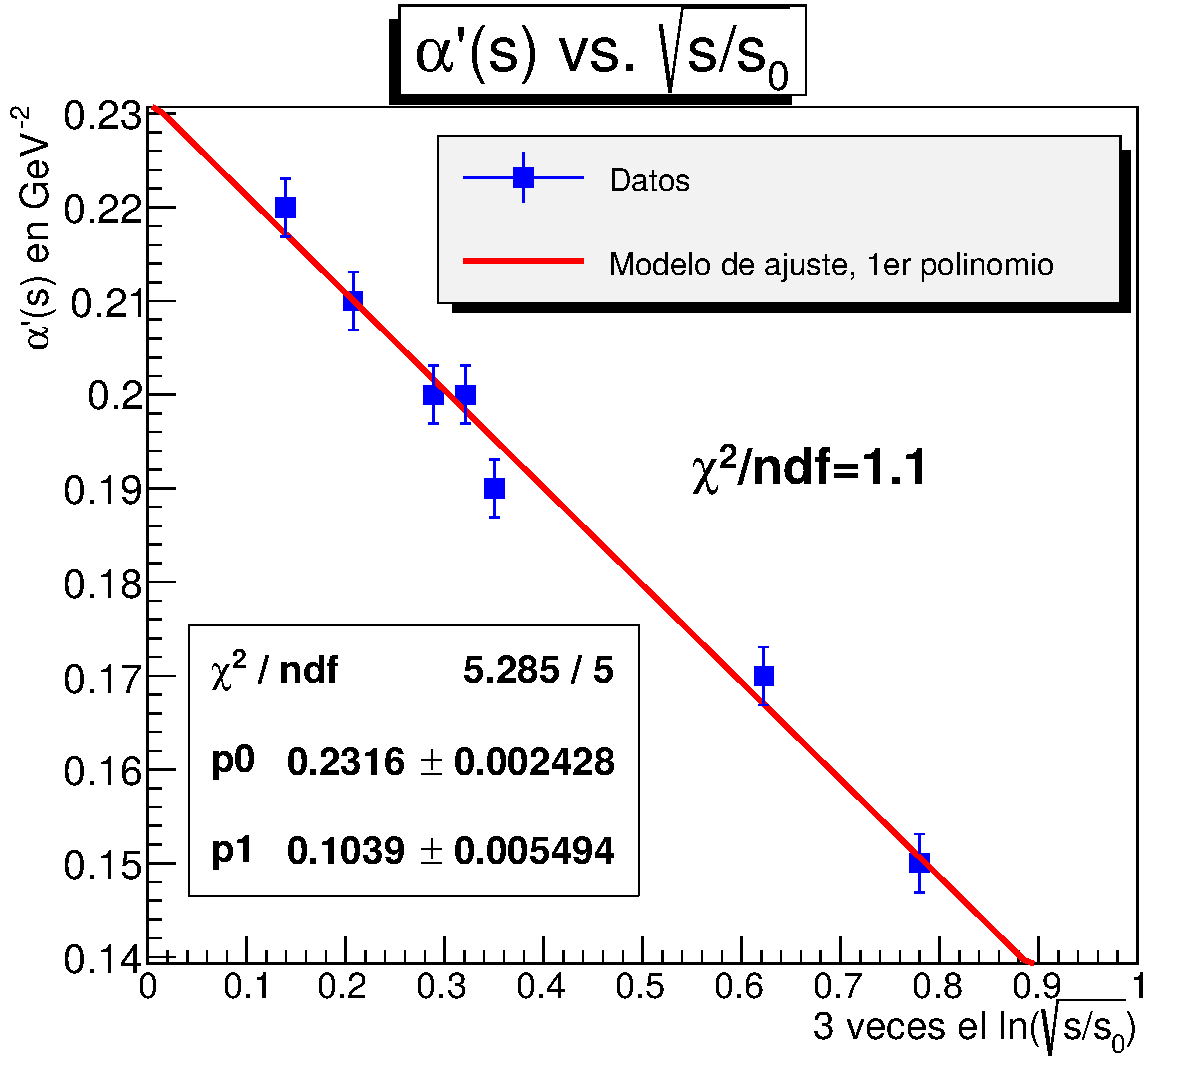
\includegraphics[width=8.5cm]{Imagenes/figurastesis/graficas/pendientepomeron.pdf}
\caption{\mismall La dependencia de $\alpha'$ en GeV$^{-2}$ del logaritmo del logaritmo del logaritmo de $\left(\sqrt{s/s_{0}}\right)$.}
\label{lafig5_18}
\end{figure}

\begin{equation}
\label{ecuacioPendientepomeron}
\alpha'(s)=(0\textup{.}232\pm 0\textup{.}002)-
(0\textup{.}104\pm 0\textup{.}006) \ln\ln\ln\left(\sqrt{s/s_o}\right)
\end{equation}

\begin{table}[H]
\begin{center}
\caption{\mismall Se muestran los valores obtenidos de $\alpha'$ usados en los ajustes en colisiones prot\'on(antiprot\'on)-prot\'on.}
\label{table0}
\begin{tabular}{c c c}\\
\noalign{\hrule height 0.5pt}
\toprule % <-- Toprule here
$\sqrt{s}$(GeV)& $ \alpha'(s)$(GeV$^{-2}$)\\ 
\hline 
23.5 & 0.22 $\pm$ 0.003 \\ 
 
30.7 & 0.21 $\pm$ 0.003 \\ 
 
44.7 & 0.20 $\pm$ 0.003 \\ 

53.0 & 0.20 $\pm$ 0.003 \\ 

62.5 & 0.19 $\pm$ 0.003 \\ 

7000 & 0.15 $\pm$ 0.003 \\ 
   
630  &   0.17 $\pm$ 0.031\\
\bottomrule % <-- Bottomrule here
\noalign{\hrule height 0.5pt}
 \end{tabular}
\end{center}
\end{table}